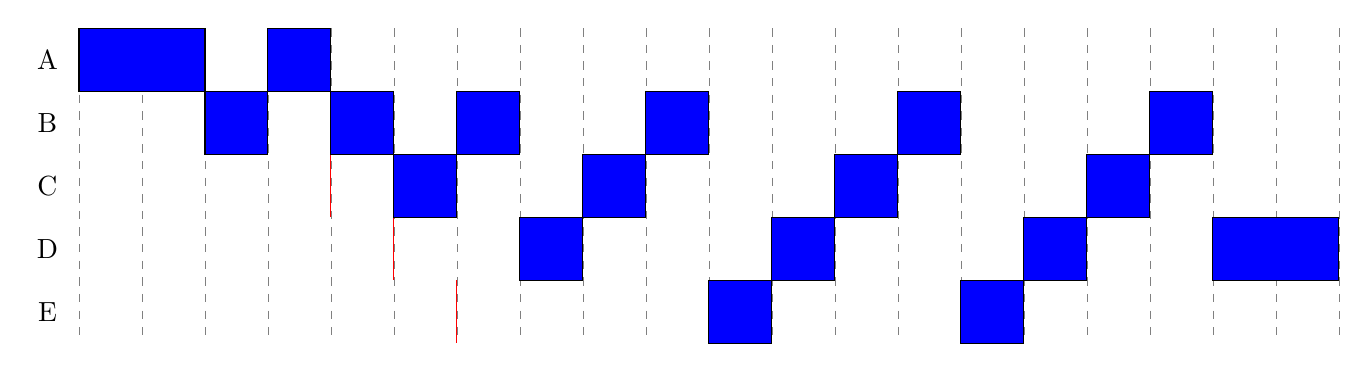
\begin{tikzpicture}[scale=.8]
   \foreach \i in {0,...,20}
   \draw[dashed, help lines] (\i,0) -- (\i,-5);

   \node (A) at (-.5,-.5) {A};
   \node (B) at (-.5,-1.5) {B};
   \node (C) at (-.5,-2.5) {C};
   \node (D) at (-.5,-3.5) {D};
   \node (E) at (-.5,-4.5) {E};

   \foreach \p in {0,...,4}
   \draw[red] (2+\p, -\p) --++ (0,-1);


   \draw[fill=blue] (0,0) rectangle (2,-1) rectangle (3,-2) (3,0) rectangle (4,-1);
   \draw[fill=blue] (4,-1) rectangle (5,-2) rectangle (6,-3) (6,-1) rectangle (7,-2);
   \draw[fill=blue] (7,-4) rectangle (8,-3) rectangle (9,-2) rectangle (10,-1);
   \draw[fill=blue] (10,-5) rectangle (11,-4) rectangle (12,-3)
                           rectangle (13,-2) rectangle (14,-1);
   \draw[fill=blue] (14,-5) rectangle (15,-4) rectangle (16,-3)
                           rectangle (17,-2) rectangle (18,-1);
   \draw[fill=blue] (18,-4) rectangle (20,-3);

\end{tikzpicture}

   % Tt     4  18 17 20 15 //
   % Tr     4  16 13 14 7 10.8
   % Tr/Ts  4/3 8/3 13/4 14/5 7/2 2.71
